\documentclass[10pt, a4paper]{article}
\usepackage[a4paper]{geometry}
\usepackage[utf8]{inputenc}
\usepackage{amsmath,amsthm,amssymb,xfrac}
\usepackage{fancyhdr}
\usepackage[hungarian]{babel}
\usepackage{graphicx}
\usepackage{float}
\usepackage{comment}
\usepackage{siunitx}
\usepackage{hyperref}
\usepackage{siunitx}
\usepackage{natbib}
\usepackage{empheq}
\usepackage{wrapfig}
\usepackage{chngcntr}
\usepackage{physics}
\usepackage{mathtools}
\counterwithin{figure}{section}
\usepackage{titlesec}
\usepackage{dsfont}
\usepackage{pdfpages}
\usepackage{t1enc}
\usepackage{tabto}
\graphicspath{ {./images/} }


\newcommand{\N}{\mathbb{N}}
\newcommand{\Z}{\mathbb{Z}}
\newcommand{\R}{\mathbb{R}}
\newcommand{\Q}{\mathbb{Q}}

\newcommand{\adat}{\begin{trivlist}\item[\hskip \labelsep {\bfseries 
			{Adatok:}}]\end{trivlist}}
\newcommand{\egy}{\begin{trivlist}\item[\hskip \labelsep {\bfseries 
			{1. Feladat:}}]\end{trivlist}}
\newcommand{\ketto}{\begin{trivlist}\item[\hskip \labelsep {\bfseries 
			{2. Feladat:}}]\end{trivlist}}
\newcommand{\harom}{\begin{trivlist}\item[\hskip \labelsep {\bfseries 
			{3. Feladat:}}]\end{trivlist}}
\newcommand{\negy}{\begin{trivlist}\item[\hskip \labelsep {\bfseries 
			{4. Feladat:}}]\end{trivlist}}		
\newcommand{\ot}{\begin{trivlist}\item[\hskip \labelsep {\bfseries 
			{5. Feladat:}}]\end{trivlist}}
\newcommand{\hatodik}{\begin{trivlist}\item[\hskip \labelsep {\bfseries 
			{6. Feladat:}}]\end{trivlist}}
\newcommand{\het}{\begin{trivlist}\item[\hskip \labelsep {\bfseries 
			{7. Feladat:}}]\end{trivlist}}
\newcommand{\into}[2]{(#1)$\xrightarrow{}$(#2):}
\newcommand{\knm}{\;\mathrm{\left[kNm\right]}}
\newcommand{\kn}{\;\mathrm{\left[kN\right]}}
\newcommand{\meter}{\mathrm{\left[m\right]}}
\newcommand{\pknm}{\mathrm{\left[kN/m\right]}}
\newcommand{\mm}{\mathrm{\left[mm\right]}}
\newcommand{\minegy}{\mathrm{\left[10^{-4}\right]}}
\newcommand{\dimnel}{\mathrm{\left[-\right]}}
\newcommand{\fok}{\mathrm{\left[^\circ\right]}}
\newcommand{\gpa}{\mathrm{\left[GPa\right]}}

\pagestyle{fancy}
\fancyhf{}
\cfoot{\thepage. oldal}
%\rhead{\thepage. oldal\\ }
\lhead{\textbf{Szilárdságtan 2. Házi feladat}
	\\Kindlik Dániel
	\\AHU27Z
	\tabto{250pt}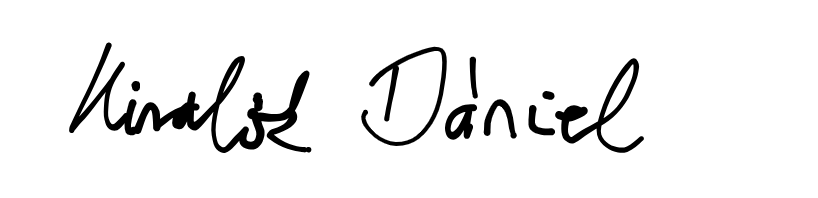
\includegraphics[width=175pt]{ alairas.png }}
\setlength{\headheight}{4em} 
\setlength{\parskip}{0.22em} 

\begin{document}
	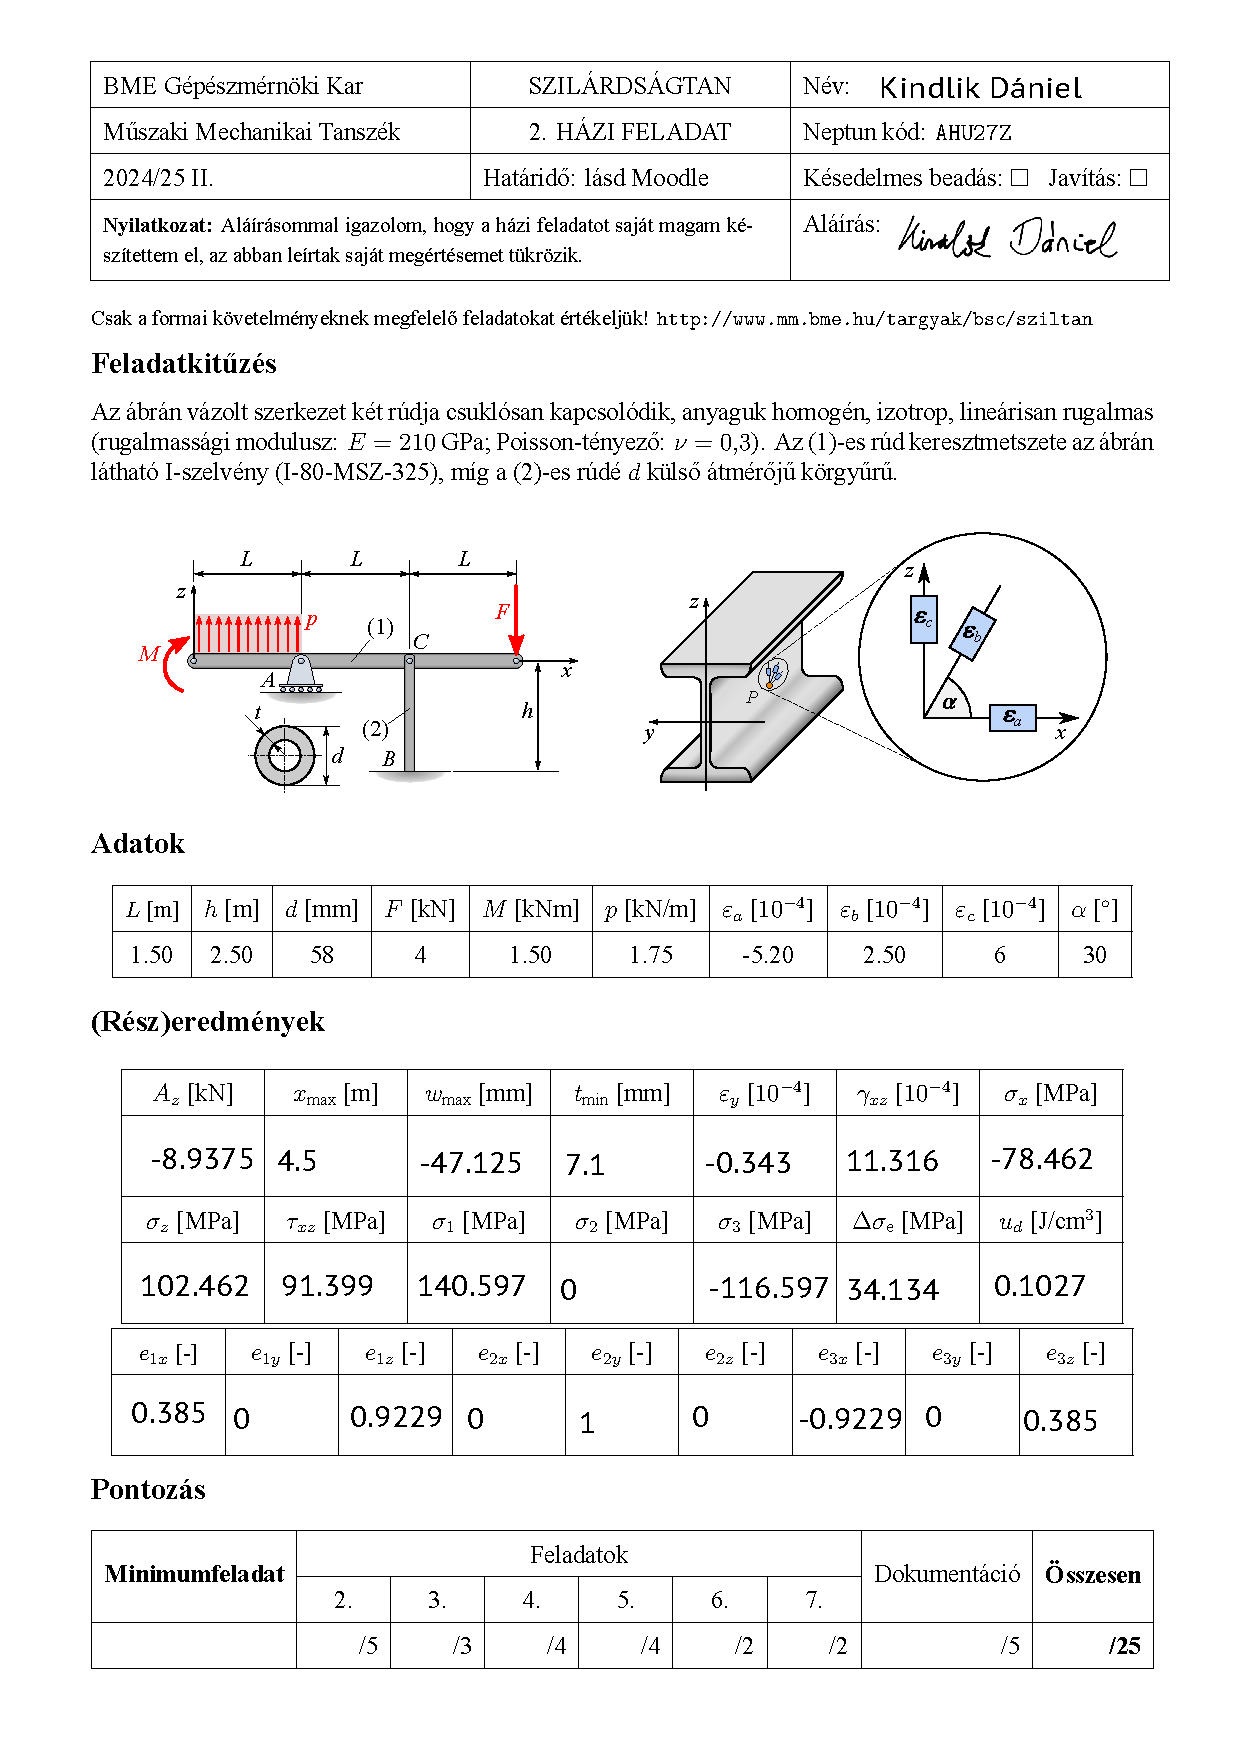
\includepdf[pages=1]{elolap.pdf}
	\adat
	$ L = 1.5\;\meter \;\;\;$ $ h = 2.5\;\meter \;\;\;$ $ d = 58\;\mm$\\\\
	$ F = 4\;\kn \;\;\; $ $ M = 1.5\knm $ $ p = 1.75\;\pknm \;\;\;$\\\\
	$ \epsilon_A = -5.2\;\minegy \;\;\;$ $ \epsilon_B = 2.5\;\minegy \;\;\;$ $ \epsilon_C = 6\;\minegy \;\;\;$ $ \alpha = 30\;\fok \;\;\;$\\\\
	$ E = 210\;\gpa \;\;\;$ $ \nu = 0.3\;\dimnel \;\;\;$
	\setcounter{page}{1}
	\egy
	\begin{center}
		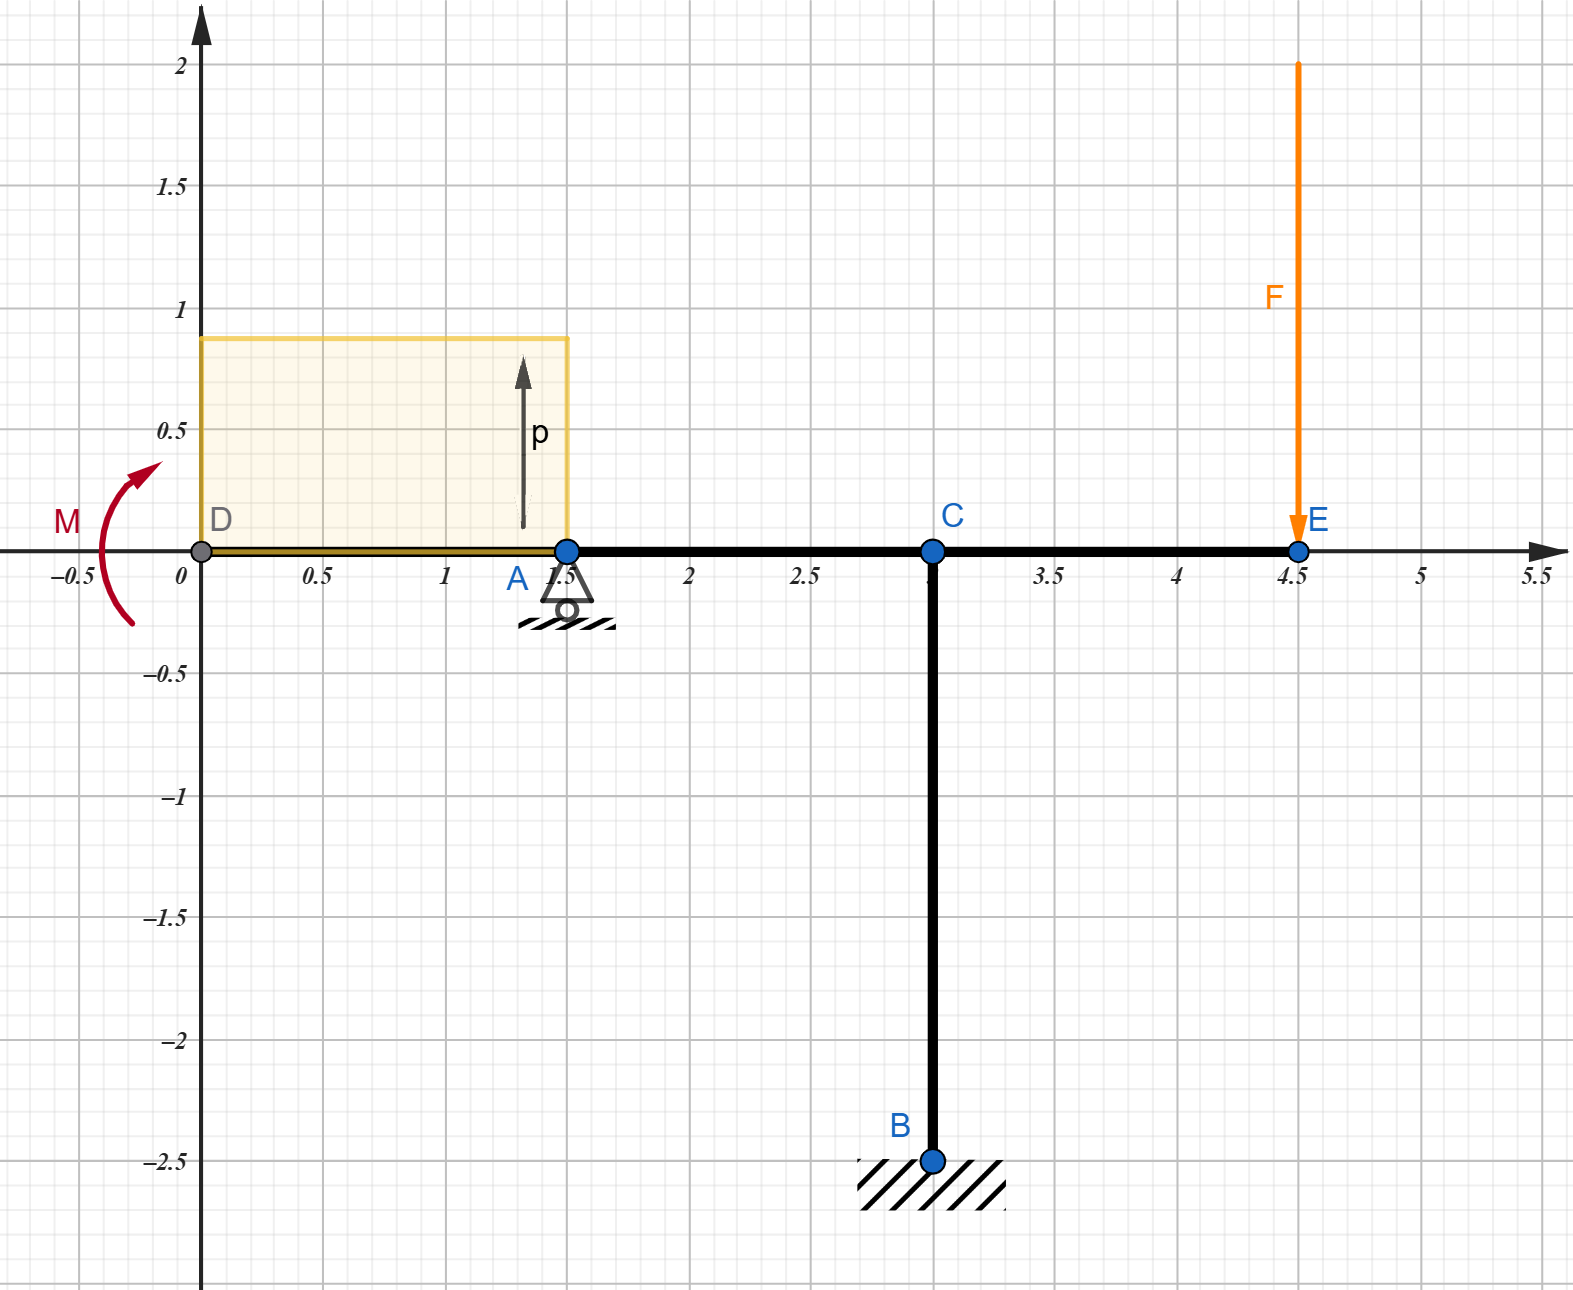
\includegraphics[width=200pt]{ meretarany.png }\\
		Az ábrán egy egység megfelel 1 m-nek és 2 kN-nak
	\end{center}
	A szerkezetünket két részre tudjuk bontani, hogy ki tudjuk számolni a reakcióerőket.\\
	Ekkor C-pontban meg fog jelenni egy C vektor, és a két rúdra külön tudunk 3-3 egyensúlyi-egyenletet írni.
	A két rész (1. eset balra, 2. eset jobbra) szabadtest-ábrája:
	\begin{center}
		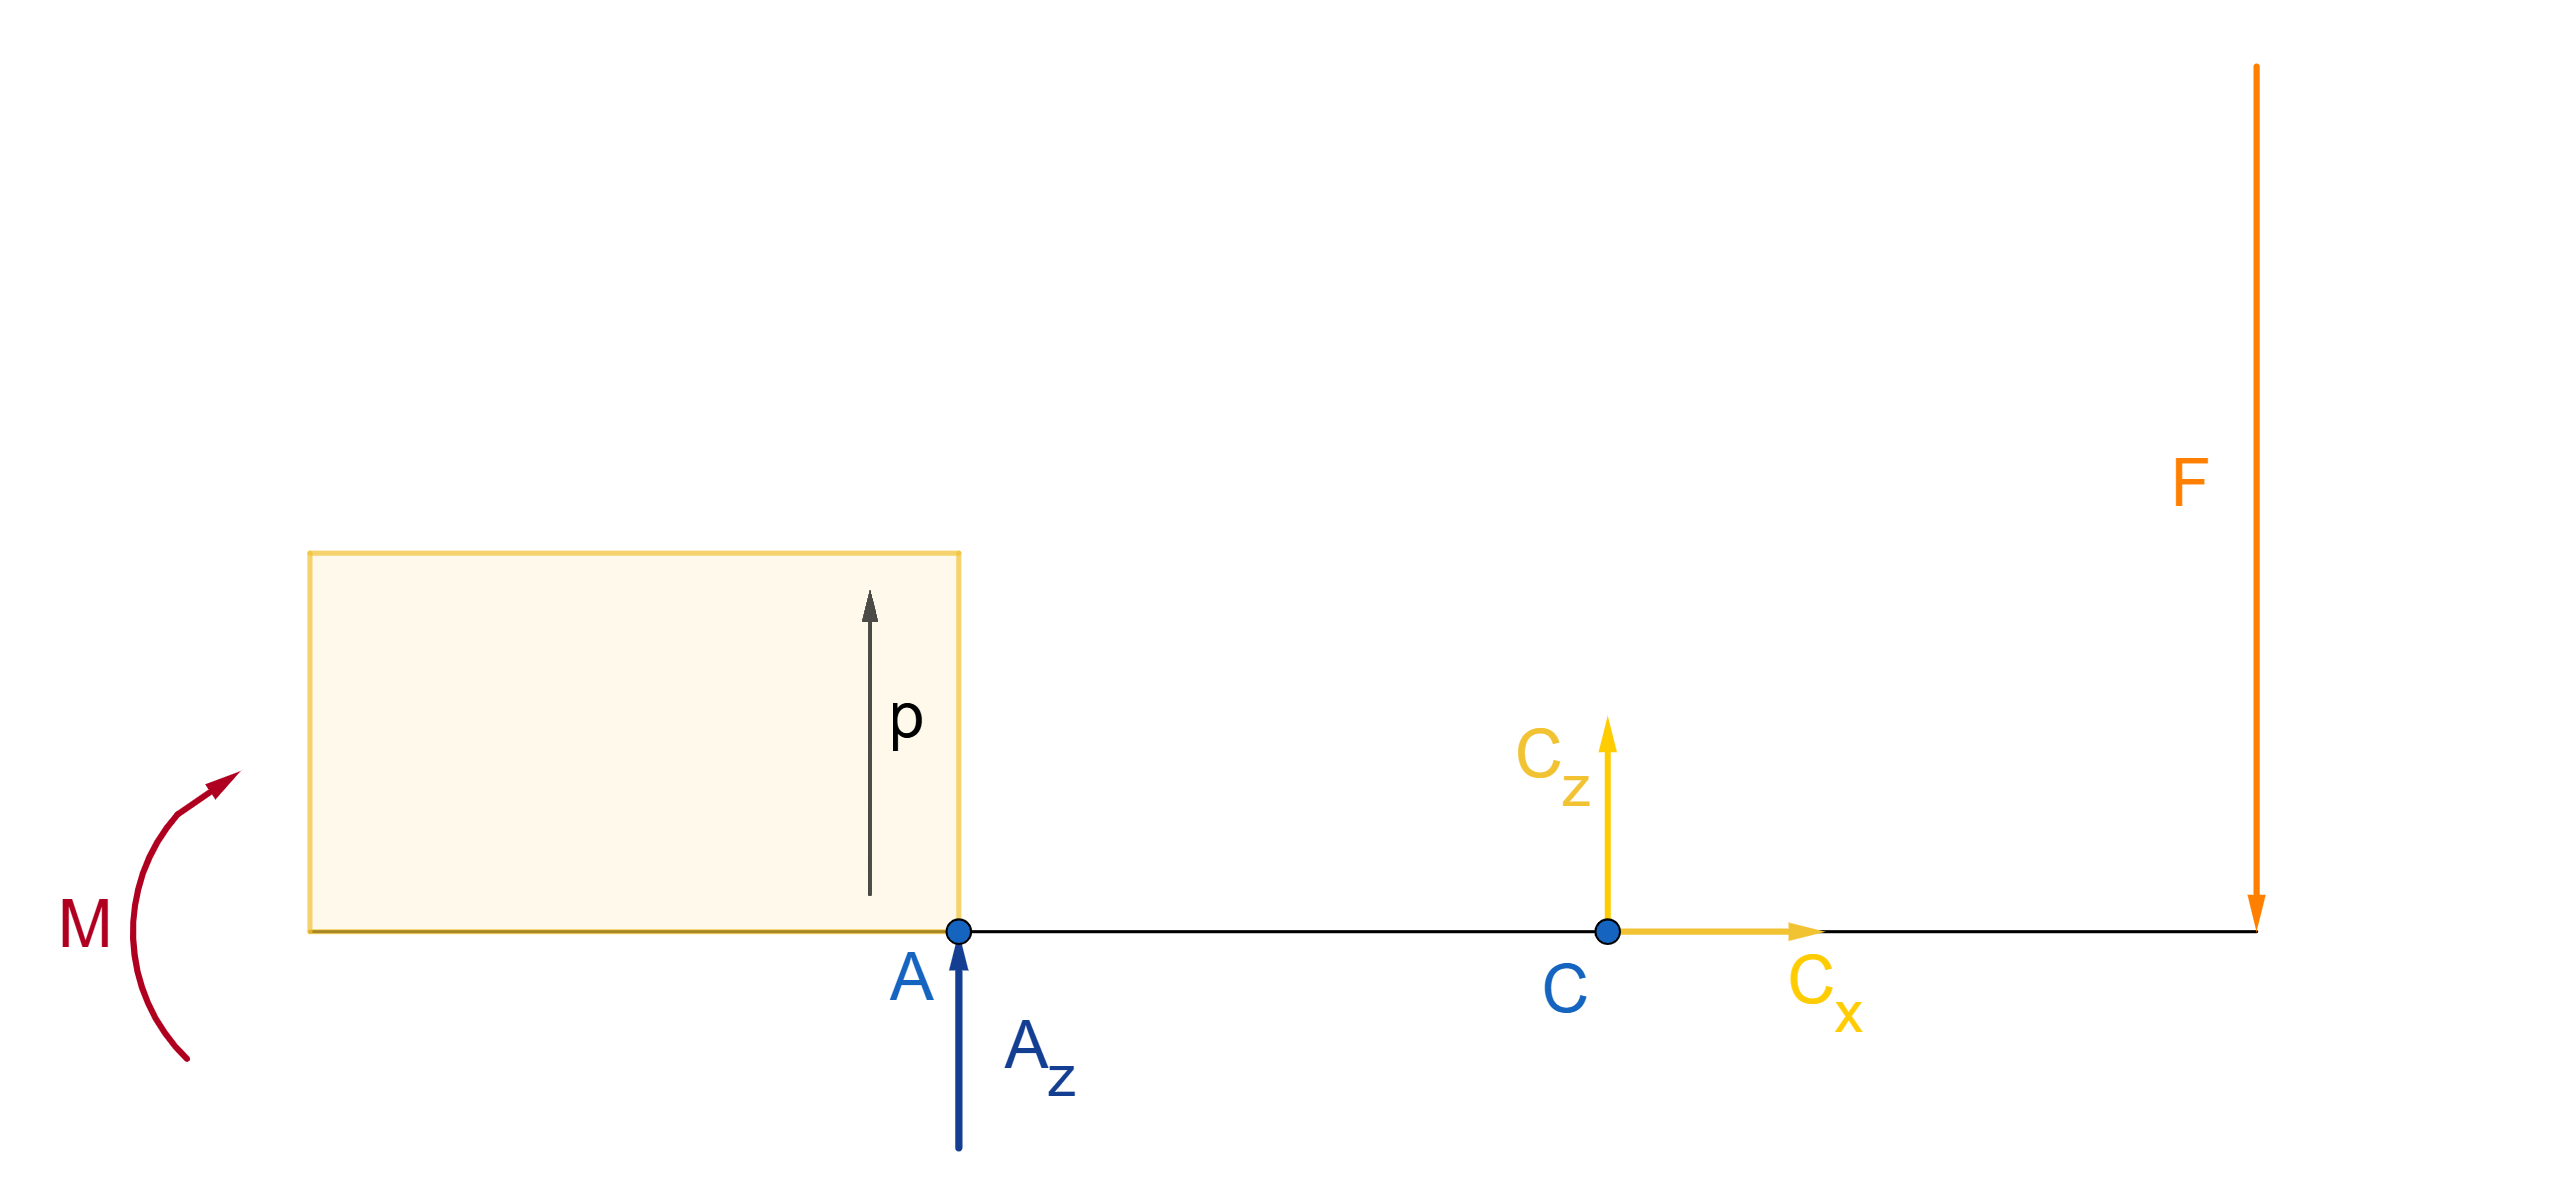
\includegraphics[width=270pt]{ SZTA1.png }
		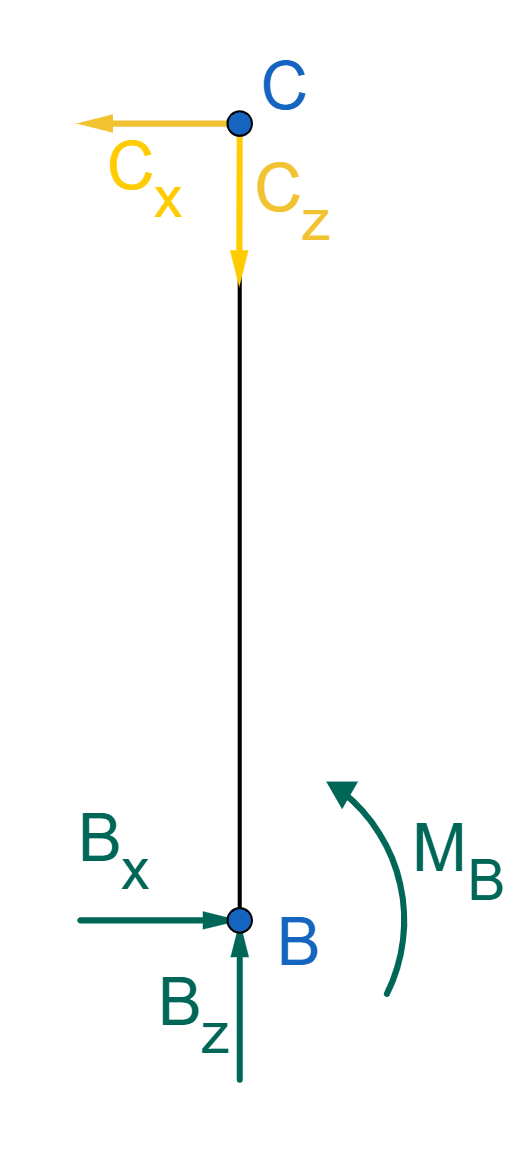
\includegraphics[width=70pt]{ SZTA2.png }
	\end{center}
	$ $\\\\\\\\
	1. esetben kijövő egyensúlyi egyenletek A pontra vonatkoztatva:\\\\
	\tabto{50pt}(1) $\sum{F_x} = 0 = C_x$\\\\
	\tabto{50pt}(2) $\sum{F_y} = 0 = A_z + C_z + p \cdot L - F$\\\\
	\tabto{50pt}(3) $\sum{M_{A'}} = 0 = C_z \cdot L - M - F \cdot 2L - (p \cdot L) \cdot \frac{L}{2}$\\\\
	2. esetben kijövő egyensúlyi egyenletek B pontra vonatkoztatva:\\\\
	\tabto{50pt}(4) $\sum{F_x} = 0 = -C_x + B_x$\\\\
	\tabto{50pt}(5) $\sum{F_y} = 0 = -C_z + B_z$\\\\
	\tabto{50pt}(6) $\sum{M_B} = 0 = M_B + B_x \cdot h$\\\\
	A két egyenletrendszer megoldása:\\\\
	\tabto{50pt}$A_z = \underline{\underline{-8.9375 \kn}}$\\\\
	\tabto{50pt}$B_x = \underline{\underline{0 \kn}}$\\\\
	\tabto{50pt}$B_z = \underline{\underline{10.3125 \kn}}$\\\\
	\tabto{50pt}$M_B = \underline{\underline{0 \kn}}$\\\\
	\tabto{50pt}$C_x = \underline{\underline{0 \kn}}$\\\\
	\tabto{50pt}$C_z = \underline{\underline{10.3125 \kn}}$
	\newpage
	\ketto
	Ahhoz hogy meg tudjuk határozni w(x)-et először meg kell adnunk az (1)-es rúd hajlítónyomatéki igénybevételét:
	A szerkezetet három részre tudjuk bontani, így a függvény:
	\begin{table}[h]
		\renewcommand{\arraystretch}{1.8}
		\resizebox{\textwidth}{!}{%
			\centering
			\begin{tabular}{c|c|c|c}
				&\begin{tabular}[c]{@{}c@{}}I.\\ $0 < x < 1.5$\end{tabular}&
				\begin{tabular}[c]{@{}c@{}}II.\\ $1.5 < x < 3$\end{tabular}&
				\begin{tabular}[c]{@{}c@{}}III.\\ $3 < x < 4.5$\end{tabular} \\ \hline
				$ \text{M}_h$&
				\begin{tabular}[c]{@{}c@{}}$- M - p \cdot x \cdot \dfrac{x}{2} =$\\ $= -0.875x^2 - 1.5 \knm$\end{tabular}&
				\begin{tabular}[c]{@{}c@{}}$- M - p \cdot L \cdot (x - \dfrac{L}{2}) - A_z \cdot (x - L)=$\\ $= 6.315x - 12.9375 \knm$\end{tabular}&
				\begin{tabular}[c]{@{}c@{}}$- M - p \cdot L \cdot (x - \dfrac{L}{2}) - A_z \cdot (x - L) - C_z \cdot (x - 2L)=$\\ $= 18 - 4x \knm$\end{tabular} \\
			\end{tabular}%
		}
	\end{table}\\\\
	Az egyenletekből adódó függvény:
	\begin{center}
		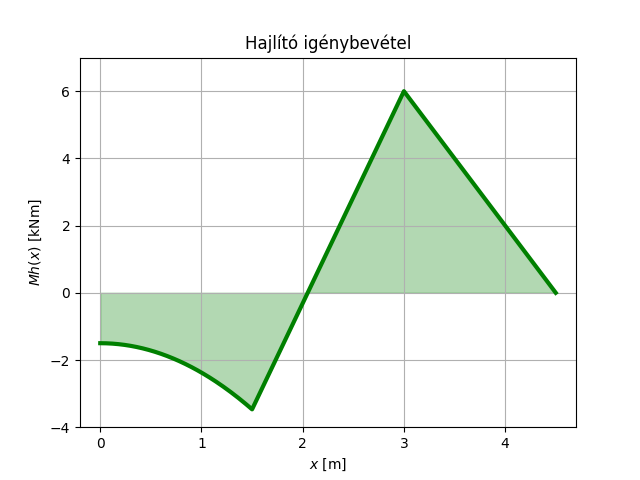
\includegraphics[width=70pt]{ hajlito.png }
	\end{center}
	Az (1)-es rúd lehajlásfüggvényének meghatározásához felhasználhatjuk az alábbi összefüggéseket:\\\\
	$-I \cdot E \cdot w''(x) = M_h(x) \xrightarrow{} -I \cdot E \cdot w'(x) = \int M_h(x) \xrightarrow{} -I \cdot E \cdot w(x) = \iint M_h(x)$\\\\
	Ezek az összefüggések a rúd egészén igazak, úgyhogy felírom a hajlítónyomaték-függvény három szakaszának szükséges alakjait:
		\begin{table}[h]
		\renewcommand{\arraystretch}{1.8}
		\resizebox{\textwidth}{!}{%
			\centering
			\begin{tabular}{c|c|c|c}
				&I.&II.&III. \\ \hline
				$ M_h$&
				$-0.875x^2 - 1.5$&
				$6.315x - 12.9375$&
				$18-4x$ \\ \hline
				$ \int M_h$&
				$-0.2917x^3 - 1.5x + C_{11}$&
				$3.15625x^2 - 12.9375x + C_{21}$&
				$-2x^2 + 18x + C_{31}$ \\ \hline
				$ \iint M_h$&
				$-0.072917x^4 - 0.75x^2 + C_{11}x + C_{12}$&
				$1.052083x^3 - 6.46875x^2 + C_{21}x + C_{22}$&
				$-0.667x^3 + 9x^2 + C_{31}x + C_{32}$\\
			\end{tabular}%
		}
	\end{table}\\
	Az egyenletekben az integrálás miatt megjelenő ismeretleneket a peremfeltételekből kijövő egyenletrendszerrel tudjuk kiszámolni, itt elhagyhatjuk a $-I \cdot E$ szorzót.\\\\
	A peremfeltételek:\\\\
	$w_1(L) = 0 \quad w_2(L) = 0 \quad w_2(2L) = 0 \quad w_3(2L) = 0 \quad w'_1(L) = w'_2(L) \quad w'_2(2L) = w'_3(2L)$\\\\
	Ezek alapján be tudunk helyettesíteni az x-ek helyére számokat, és 6db egyenletünk jön ki.\\\\\\
	Az egyenletrendszer megoldása:\\\\
	$C_{11} = 3.4688 \;\; C_{12} = -3.1465 \;\; C_{21} = 12.539 \;\; C_{22} = -7.8047 \;\; C_{31} = -33.8672 \;\; C_{32} = 38.6016$\\\\
	Az így kijövő eredményeket fel tudjuk használni $w(x)$ és $\phi(x)$függvény meghatározásához:\\\\
	$w(x) = -\dfrac{1}{I \cdot E} \cdot \iint M_h(x) \quad\quad \phi(x) = -\dfrac{1}{I \cdot E} \cdot \int M_h(x)$
		\begin{table}[h]
		\renewcommand{\arraystretch}{1.8}
		\resizebox{\textwidth}{!}{%
			\centering
			\begin{tabular}{c|c|c|c}
				&\begin{tabular}[c]{@{}c@{}}I.\\ $0 < x < 1.5$\end{tabular}&
				\begin{tabular}[c]{@{}c@{}}II.\\ $1.5 < x < 3$\end{tabular}&
				\begin{tabular}[c]{@{}c@{}}III.\\ $3 < x < 4.5$\end{tabular} \\ \hline
				$ w(x)$&
				$xyzsfdsfdsdsfdsfdfssssssssss$&
				$xyz$&
				$xyz$ \\ \hline
				$ \phi(x)$&
				$xyz$&
				$xyz$&
				$xyz$ \\
			\end{tabular}%
		}
	\end{table}\\\\
	kurva jó diagramok lestestotsostogooooooooooooooooo\\\\
	Az ábráról láthatjuk, hogy a legnagyobb lehajlás $x = 4.5$-nél következik be:\\\\
	$x_{max} = \underline{\underline{4.5 \meter}} \quad w_{max} = w(4.5) = \underline{\underline{-47.12 \meter}}$
	\newpage
	\harom
\end{document}